% make sure to download following files before compiling-
% tikzlibrarynode-families.code.tex
% tikzlibrarypositioning-plus.code.tex
% please keep the above files in the same directory
\documentclass[border=2pt]{standalone}
\usepackage{tikz}

\usetikzlibrary{shapes.geometric,backgrounds,positioning-plus,node-families,calc}
\tikzset{
  basic box/.style = {
    shape = rectangle,
    align = center,
    draw  = #1,
    fill  = #1!25,
    %font  = \large,
    rounded corners},
  header node/.style = {
    %Minimum Width = header nodes,
    %font          = \Large\bf,
    %text depth    = +0pt,
    fill          = white,
    draw},
  header/.style = {%
    inner xsep = +1.0em,
    inner ysep = +0.8em,
    append after command = {
      \pgfextra{\let\TikZlastnode\tikzlastnode}
      node [header node] (header-\TikZlastnode) at (\TikZlastnode.north) {#1}
      node [span = (\TikZlastnode)(header-\TikZlastnode)]
        at (fit bounding box) (h-\TikZlastnode) {}
    }
  },
  hv/.style = {to path = {-|(\tikztotarget)\tikztonodes}},
  vh/.style = {to path = {|-(\tikztotarget)\tikztonodes}},
  fat blue line/.style = {ultra thick, blue}
}

% set sans-serif http://tex.stackexchange.com/a/4888
\tikzstyle{every picture}+=[font=\sffamily]
\def \scaling {3.5cm}
\begin{document}

\begin{tikzpicture}[every node/.style={transform shape}, thick, >=latex, node distance=0.5cm]
	\node[basic box = blue, header = Teaching Phase] (teaching) {
		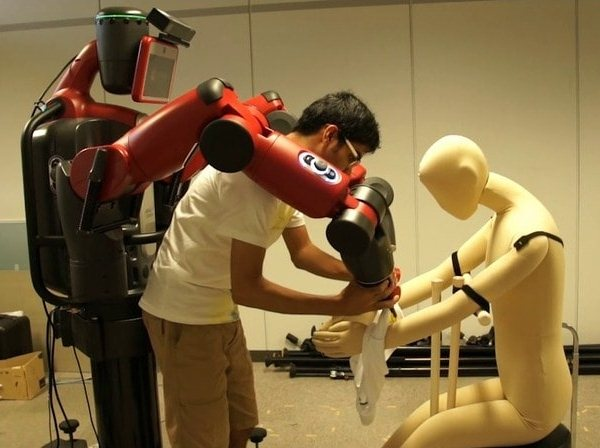
\includegraphics[height=\scaling]{teaching}%\\
		%A demonstration is performed by moving the \\
		%Baxter arms in the appropriate trajectory
	};
				
	%\node[north right = of teaching, basic box = orange, header = Trajectory Parameterization] (dmp)
	\node[north right = of teaching, basic box = orange, header = Learn Trajectory] (dmp) {
		%Baxter Left Arm Trajectory\\
		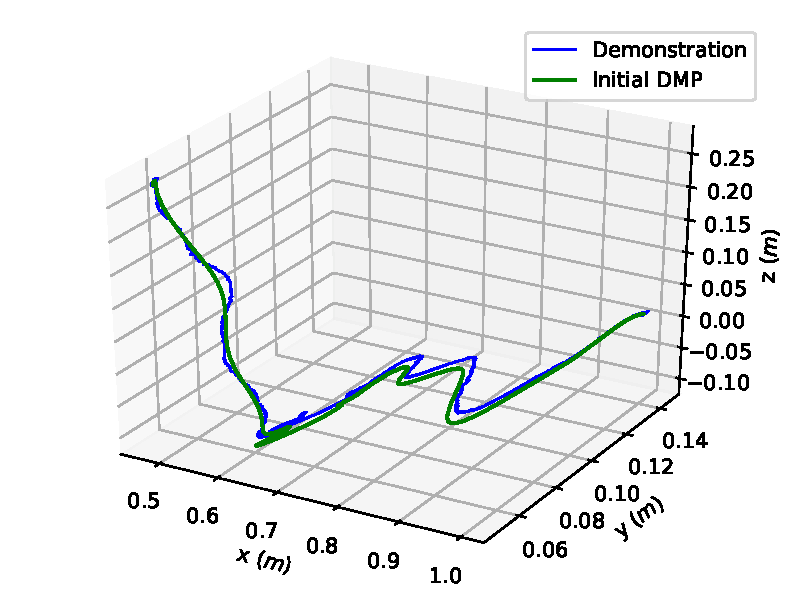
\includegraphics[height=\scaling]{dmp_init}%\\
		%Recorded trajectory is parameterized by DMP
	};
					
	\node[north right = of dmp, basic box = green, header = Testing Phase] (testing) {
		%Modified Posture\\
		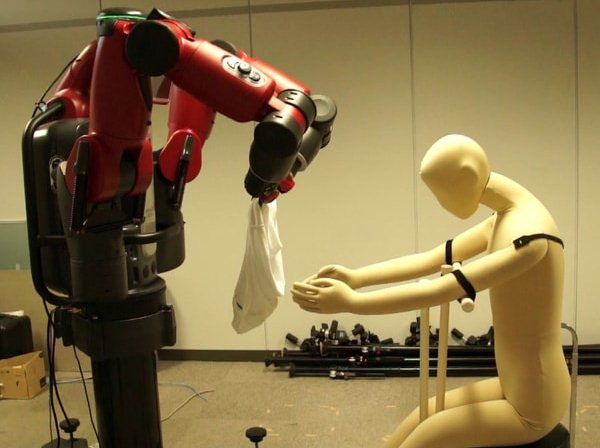
\includegraphics[height=\scaling]{testing}%\\
		%DMP can accomodate new posture
	};
				
	\node[north right = of testing, basic box = red, header = DMP Generalization] (generalization){
		%DMP Trajectory\\
		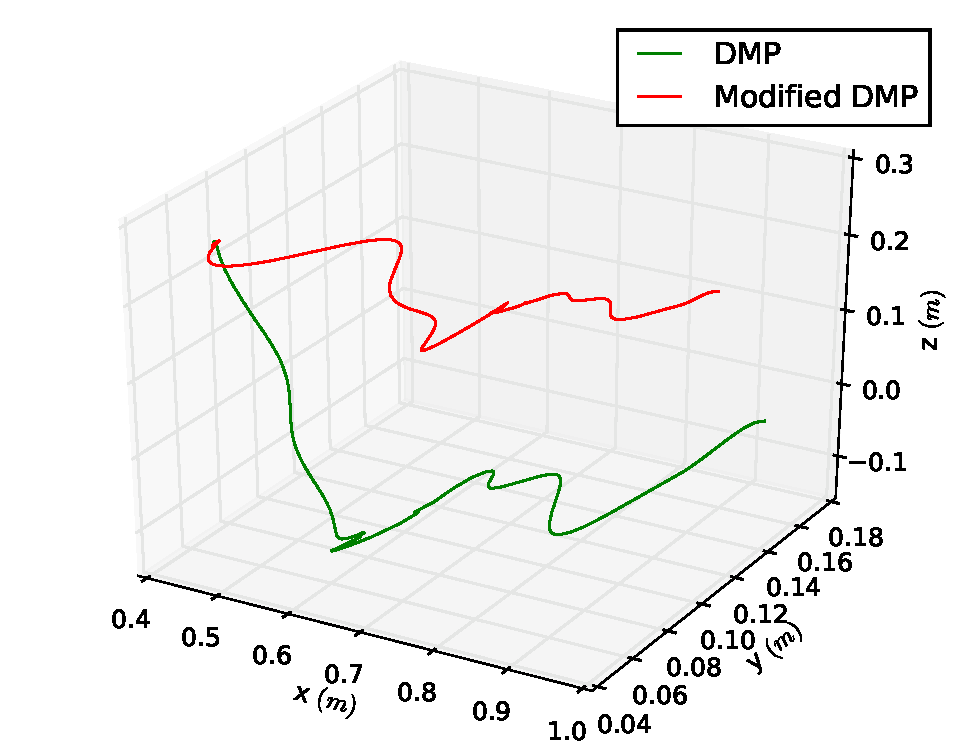
\includegraphics[height=\scaling]{dmp_mod}
	};
				
	\path[ultra thick, blue,  ->](teaching) edge[->] (dmp);
	\path[ultra thick, orange,->](dmp) edge[->] (testing);
	\path[ultra thick, green, ->](testing) edge[->] (generalization);
\end{tikzpicture}
\end{document}